%avoid page number on blank pages when cleared
\thispagestyle{empty}
\cleardoublepage
\chapter{Marco Te\'orico}
\label{sec:dev}
\section{Endrov}
\label{sec:endrov}

\emph{Endrov}, es una arquitectura de extensiones de c\'odigo abierto,
dirigida al an\'alisis de im\'agenes y procesamiento de datos.
Se encuentra implementada en \emph{Java}, es portable, y puede ser ejecutada localmente o como 
un \emph{applet}, como se indica en \cite{web:endrov}. \emph{Endrov} surgi\'o
de la necesidad de un software avanzado de c\'odigo abierto que permitiese procesar 
los complejos datos espacio-temporales presentes en im\'agenes de microscopios, 
utilizadas en la investigaci\'on biol\'ogica.\\

\emph{Endrov}, tiene como objetivo mejorar las funcionalidades del software c\'odigo abierto
de an\'alisis de im\'agenes \emph{ImageJ}, proveyendo un dise\~no mas moderno. 
Las deficiencias principales de \emph{ImageJ} son: falta de soporte de metadatos,
no existe soporte real de 5D, la arquitectura de extensiones es confusa, las vistas
no pueden ser extendidas fácilmente, y el procesamiento de lotes es complicado, 
tal como se indica en \cite{web:endrovhome}.
Otros problemas que inspiraron la creaci\'on de \emph{Endrov} fueron: la ausencia de un 
formato de im\'agen estandarizado, y la dificultad
de almacenar datos complejos en los formatos abiertos que existen actualmente.
El grupo de desarrollo cre\'o el formato OST para manejar grandes conjuntos de im\'agenes.
Puede almacenar todo tipo de informaci\'on, pero se encuentra optimizado para im\'agenes.\\

\emph{Endrov}, es tanto una liber\'ia como un programa de an\'alisis y procesamiento de 
im\'agenes. El dise\~no se realiz\'o haciendo fuerte enf\'asis en separar el c\'odigo
de la interfaz gr\'afica de los tipos de datos, filtros y otras extensiones para 
procesamiento de datos. La idea del programa es proveer una herramienta robusta para
an\'alisis y procesamiento de im\'agenes que pueda cubrir las necesidades de aquellos
laboratorios, grupos de investigacion y cualesquiera otros tipos de usuario, que 
manipulan im\'agenes diariamente, \cite{web:endrov}.\\

\emph{Endrov} fue desarrollado por el \emph{TBU Group} del Instituto Karolinska en Suecia, y 
fue liberado oficialmetnte el 17 de Junio de 2009, bajo la licensia BSD.


\section{M\'etodo del valor umbral}
\label{sec:thresholding}

Los m\'etodos del valor umbral (MVU), mejor conocidos por su nombre en ingles: \emph{thresholding},
son un conjunto de algoritmos para segmentar gr\'aficos rasterizados, que permiten separar
objetos presentes en una im\'agen del resto. Esta segmentaci\'on es usualmente representada
a trav\'es de una im\'agen binaria, que se obtiene despu\'es de procesar la im\'agen original 
en escala de grises.\\

Una imagen binaria es un tipo de imagen discreta, en la cual cada pixel tiene asignado uno de
dos valores posibles (tipicamente $1$ o $0$). Cada valor indica si el pixel
pertenece al primer o segundo plano (fondo) de la im\'agen original, respectivamente.
Como se indica en \cite{web:thresholding}, durante la ejecuci\'on de un m\'etodo del valor
umbral, se marcan pixeles individuales como p\'ixeles objeto o pixeles de fondo, seg\'un
corresponda. Asumiendo que los objetos en las im\'agenes son mas brillantes que el fondo,
un pixel se marca como pixel objeto si su valor de luminosidad (u otro valor unidimensional) 
es mayor que un valor umbral determinado, de otro modo se marca como pixel de fondo.
Esta conveci\'on se denomina \emph{umbral por encima}. Diferentes variantes incluyen:
\emph{umbral por debajo}, que es el opuesto al anterior; \emph{umbral por dentro}, donde un
pixel es marcado como objeto si su valor de comparaci\'on se encuentra entre dos 
umbrales; y \emph{umbral por fuera}, que es el opuesto a \emph{umbral por dentro}, seg\'un
se explica en \cite{shapiro}.\\


En las aplicaciones de procesamiento de im\'agenes donde el estudio se enfoca en 
objetos particulares contenidos en una imagen, los MVU se convierten en una herramienta
sencilla para separar estos objetos del fondo, aunque no siempre precisa. En \cite[p.146]{thres},
se mencionan diversas aplicaciones en procesamiento de im\'agenes que involucran MVU, tales
como: an\'alisis de im\'agenes de documentos, donde el objetivo es extraer caracteres, logos,
contenido gr\'afico o notas musicales entre otros; procesamiento de mapas, que se centra en
encontrar l\'ineas, leyendas y caracteres; procesamiento de escenas, donde se busca detectar
un objetivo o blanco; e inspecci\'on de calidad de materiales, donde se desea delinear piezas
defectuosas, entre muchos otros.\\

El par\'ametro clave para los MVU es el valor umbral (o valores umbrales para los enfoques de
\emph{umbral por dentro} y \emph{umbral por fuera}). El valor puede ser tanto calculado
automaticamente, como establecido o ajustado manualmente. Los diferentes MVU pueden ser categorizados 
de acuerdo de la informaci\'on que explotan. En \cite[p.147]{thres}, Sezgin y Sankur
categorizan los MVU en seis gr\'upos principales: m\'etodos basados en histograma de formas,  
m\'etodos basados en agrupamiento, m\'etodos basados en entrop\'ia, m\'etodos espaciales y
m\'etodos locales.\\

En la Figura \ref{fig:thres1}, se muestran dos im\'agenes: una en escala de grises y la 
otra, la imagen binaria obtenida a trav\'es de un m\'etodo del valor umbral.

\begin{figure}[h t b p ! H]
  \centering
  \subfloat[Imagen en escala de grises]{\label{fig:threso}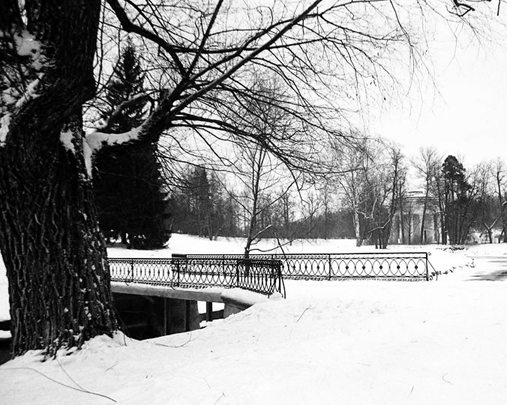
\includegraphics[width=0.45\textwidth]{thres/winter_o}}
\qquad
  \subfloat[Imagen binaria obtenida a trav\'es de un m\'etodo del valor umbral]{\label{fig:thres1}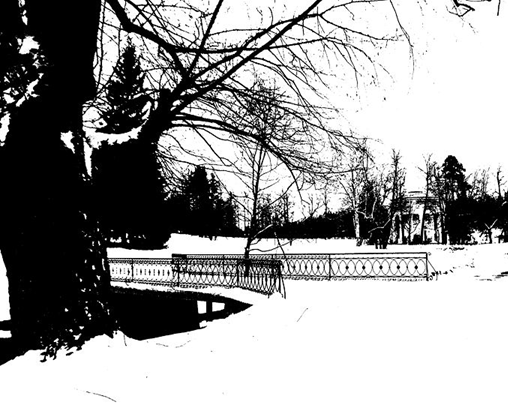
\includegraphics[width=0.45\textwidth]{thres/winter_thres}}
  \caption[Im\'agen en escala de grises antes y desp\'ues de aplicar un m\'etodo del valor umbral ]{Im\'agen en escala de grises antes y desp\'ues de 
    aplicar un m\'etodo del valor umbral. Las im\'agenes fueron tomadas de \cite{web:thresholding}}
  \label{fig:thres1}
\end{figure}

\section{Transformada de distancia}
\label{sec:dt}

Una transformada de distancia o mapa de distancias es una representaci\'on de
una imagen digital, en la cual a cada pixel de la im\'agen le corresponde
un valor que indica la distancia entre ese pixel y el pixel mas cercano que pertenezca
al fondo de la imagen. Se calcula a partir de una im\'agen binaria, que consista
en pixeles de objeto y pixeles de fondo. La imagen que se obtiene corresponde a
una especie de representaci\'on en escala de grises del primer plano de la im\'agen
binaria (conformado por los objetos).\\
El valor mapeado para cada pixel, depende directamente de la funci\'on de distancia,
que define el patron de medici\'on de distancia entre pixeles de la imagen. Existen
diversas funciones de distancia tales como: \emph{Manhattan},
\emph{tablero de ajedrez}, \emph{Euclideana}, \emph{Chamfer 3-4} y \emph{Octogonal}, 
\cite[p.363]{dtresearch}. As\'i mismo, existen muchas otras funciones de
distancia, normalmente derivadas de las anteriormente mencionadas.
En la Figura \ref{fig:dtexamples}, se muestra el resultado de aplicar 
diferentes funciones de distancia a una imagen que contiene un punto en el centro,
rodeado por un fondo blanco.

\begin{figure}[h t b p ! H]
 \centering
   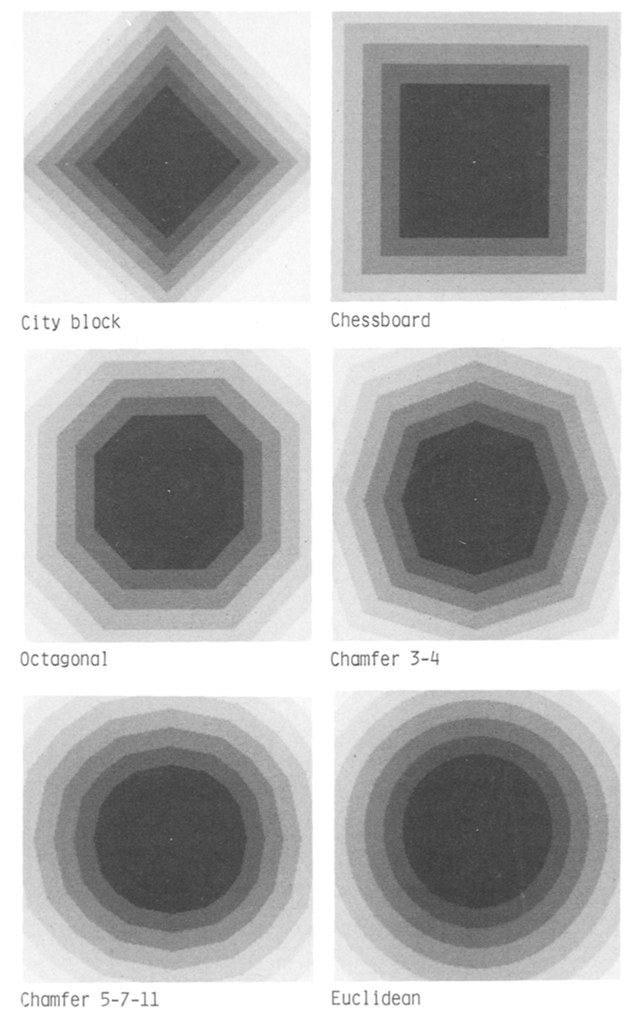
\includegraphics[scale=0.4]{dt/dtref}
 \caption[Distancias a partir de un punto para seis transformadas de distancia]{ 
   Distancias a partir de un punto para seis transformadas de distancia. Mientras 
   mas claro es el color, mas larga es la distancia \cite[p.365]{dtresearch}}
 \label{fig:dtexamples}
\end{figure}

Como se indica en \cite{dtresearch2}, las transformadas de distancia juegan un rol
central en la comparaci\'on de im\'agenes binarias, particularmente aquellas
resultantes de t\'ecnicas de detecci\'on de caracter\'isticas locales, tales 
como detecci\'on de contornos o detecci\'on de esquinas.
Las transformadas de distancia pueden ser interpretadas, tambi\'en, como
topograf\'ias de islas, donde la etiqueta o valor de cada pixel indica la altura o 
profundidad de la regi\'on. De esta forma, se pueden detectar crestas y picos, 
que constituyen la base principal de met\'odos sencillos para encontrar el 
esqueleto topol\'ogico de objetos en im\'agenes, tal como se explica en \cite[237]{ridgedt}.
Las transformadas de distancias son tambi\'en herramientas muy \'utiles para el 
mejoramiento de la eficiencia de algoritmos de morfolog\'ia, tales como: 
\emph{reducci\'on de contornos} and \emph{expansi\'on de contornos}.\\

\section{Esqueletizaci\'on}
\label{sec:skeletonization}

Un esqueleto topol\'ogico es una representaci\'on compacta y simple de un objeto, que
consiste en una versi\'on reducida o delgada del mismo, que es equidistante a sus bordes, 
y que preserva muchas de las caracter\'isticas topologicas y geom\'etricas de la
imagen original, tal como se explica en \cite{wikipedia:skeleton,ssm,augmented}. 
Por lo general, el esqueleto se define como el conjunto de los centros de los discos m\'aximos
contenidos en la imagen original, \cite{ssm,augmented}. Existen muchas otras definiciones diferentes,
que dependen, principalmente, de la forma en que el esqueleto es generado.
Independientemente de la definici\'on que se adopte, si los puntos pertenecientes al esqueleto
son calculados en relaci\'on con su distancia a los bordes originales del objeto, 
el esqueleto puede ser utilizado para reconstruir con exactitud la figura original.
La figura \ref{fig:genskeleton} presenta el esqueleto de una silueta de caballo, y la
imagen binaria a partir de la cual fue calculado el esqueleto.

\begin{figure}[h t b p ! H]
  \centering
  \subfloat[Imagen Binaria]{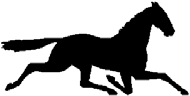
\includegraphics[scale=0.8]{skeleton/horsebinary}}
\qquad
  \subfloat[Esqueleto topol\'ogico]{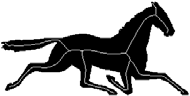
\includegraphics[scale=0.8]{skeleton/horseskeleton}}
  \caption[Imagen binaria de una figura de caballo y su esqueleto]{Imagen binaria de una figura de
caballo y su esqueleto. Im\'agenes tomadas de \cite{ssm}}
  \label{fig:genskeleton}
\end{figure}


Los esqueletos topol\'ogicos pueden ser categorizados en diferentes tipos.
Telea et al, \cite{augmented}, describen tres tipos de esqueleto de acuerdo a la forma en que
son calculados, tales como: \emph{esqueleto por reducci\'on morfol\'ogica}, 
\emph{esqueleto por m\'etodos geom\'etricos} y \emph{esqueleto por transformada de distancia}.
El m\'etodo de \emph{reducci\'on morfol\'ogica} consiste en la reducci\'on iterativa de los bordes
del objeto, identificando y marcando, capa por capa, aquellos puntos cuya remoci\'on no afecte
la topolog\'ia del objeto. Estos m\'etodos son sencillos, por lo general, aunque suelen requerir
heur\'isticas complejas para asegurar la conectividad del esqueleto, como se indica en
\cite{augmented}. En \cite{onepass} y \cite{thinning}, se describen dos enfoques paralelos
eficientes para garantizar la conectividad de esqueletos producidos a trav\'es 
\emph{reducci\'on morfol\'ogica}.\\
Los \emph{m\'etodos geom\'etricos} se centran en calcular el diagrama de Voronoi de una
representaci\'on pol\'igonal de los bordes del objeto. El diagrama de Voronoi representa
el eje medio de los bordes. Tal como se asegura en \cite[p.251]{augmented}, estos m\'etodos
producen un esqueleto conectado y preciso, pero son muy complejos de implementar, requieren
una robusta discretizaci\'on de los bordes, y son computacionalmente costosos.\\
El tercer tipo comprende los m\'etodos que calculan el esqueleto a partir de 
la transformada de distancia. El enfoque com\'un consiste en encontrar los puntos cresta
y conectarlos, \cite{maxima, euclideancentre, ridgedt}. Por lo general, estos m\'etodos
pueden garantizar que los puntos esqueletos encontrados son precisos y acertados, 
pero no la conectividad del esqueleto, ni su completitud.\\

El esqueleto topol\'ogico es una herramienta importante para la representaci\'on
y reconocimiento de objetos, en diferentes areas, tales como: visi\'on artificial,
an\'alisis de im\'agenes, y procesamiento de im\'agenes digitales, incluyendo 
reconocimiento \'optico de caracteres, reconocimiento de huellas digitales, inspecci\'on
visual, reconocimiento de patrones, compresi\'on de im\'agenes binarias y plegamiento
de proteinas, \cite{skprotein}.


\section{Ajuste de formas}
\label{sec:shapefitting}

El ajuste de formas (en ingl\'es \emph{shape matching}), es un problema
central en los sistemas de informaci\'on visual, visi\'on artificial, 
reconocimiento de patrones y rob\'otica, \cite{matchingbook}. Consiste
en identificar el area o contorno de una forma en espec\'ifico o de determinadas 
clases de formas en una im\'agen, y tiene un rol fundamental en la extracci\'on
de contenido en im\'agenes y en la recuperaci\'on de im\'agenes basada en contenido.
Tal como explica Veltkamp en \cite{matching2}, el ajuste de formas 
se ocupa de la transformaci\'on de una forma determinada y de la
medici\'on de su similitud con respecto a otra forma, utilizando
alguna medida de similitud o distancia entre formas.\\

El concepto de forma es abstracto. La mayor\'ia de los
enfoques en ajuste de formas definen las formas de manera 
geom\'etrica. Esta descripci\'on geom\'etrica puede 
consistir tanto en un conjunto de puntos, curvas, superficies,
solidos, etc, como en un patr\'on geom\'etrico dispuesto de acuerdo
a algun grupo de transformaciones geometr\'icas, en particular transformaciones
de semejanza (traslaci\'on, rotaci\'on y escala), tal como se indica en
\cite{matching2}. 

Por lo general, se utiliza un patr\'on geom\'etrico de forma, llamado
descriptor de forma, para representar la clase del objeto a ajustar.
Existen diferentes tipos de descriptores de forma, que se diferencian de acuerdo
al tipo de informaci\'on que los define y a la naturaleza del problema, (ver
Sec. \ref{sec:shapedesc}).\\

Se han desarrollado diferentes enfoques para el problema de ajuste de formas.
Esta secci\'on se centra en aquellos enfoques basados en geometr\'ia
computacional, dado que son los mas relacionados con el enfoque
seguido en este trabajo. La geometr\'ia computacional consiste en buscar y 
analizar algoritmos eficientes para resolver problemas geom\'etricos.
En \cite{matchingbook}, Veltkamp y Hagedoorn mencionan diferentes
enfoques de ajuste de formas tales como: poda de \'arboles, la transformada
de Hough generalizada, el m\'etodo de alineaci\'on, estad\'isticas,
modelos deformables, relajaci\'on de etiquetas, descriptores de Fourier,
transformada \'ondula y redes neurales. As\'i mismo, categorizan las 
t\'ecnicas de ajuste de forma en dos grupos principales:
\emph{transformadas de imagen global} y \emph{m\'etodos de objetos globales}.
El grupo de \emph{transformadas de imagen global} se refiere a las 
t\'ecnicas que ``transforman la imagen de informaci\'on de color en
el dominio espacial a variaci\'on de color en el dominio frecuencial''.
Estos enfoques no representan la forma expl\'icitamente para el ajuste,
sino que representan las transiciones de color o intensidad en
la imagen. Esto hace imposible medir las diferencias entre dos
imagenes en t\'erminos de formas, as\'i como comparar y ajustar
una forma a una parte espec\'ifica de la imagen.\\


On the other hand the \emph{global object methods} work with a complete
object area or contour and can analyze specific areas in the 
image instead of requiring processing the whole image as in 
the global image transforms. In order to perform a proper
matching, the objects in the image have to be completely and
clearly segmented. Some of these methods are: \emph{moments}, where an
object is described as a set of moments, \emph{modal matching},
where the boundary is used instead of the area and is described 
with Fourier descriptors and \emph{curvature scale space}, where a
scale space and parameterized representation of the contour of the 
objects is used.\\

Veltkamp describes in \cite{matching2} various forms in
which shape matching is studied, given two shape patterns
and a dissimilarity measure. These are:

\begin{itemize}
\item \textbf{Computation Problem: }Compute the dissimilarity
  between the two patterns
\item \textbf{Decision Problem: }
  \begin{itemize}
  \item  For a given threshold, decide
  whether the dissimilarity is smaller than the threshold.
  \item For a given threshold, decide
    whether there exists a transformation such that the
    dissimilarity between the transformed pattern and the other 
    pattern is smaller than the threshold
  \end{itemize}
 
\item \textbf{Optimization Problem: }Find the transformation
that minimizes the dissimilarity between the transformed
pattern and the other pattern.
\end{itemize}

A well studied optimization approach for shape matching is
Active Contour Models (\emph{Snakes}),  which inspired much 
of the shape fitting approach of this work 
(see Sec \ref{sec:metfit}). In \cite{snakes} a snake is defined 
as an energy-minimizing spline guided by external constraint
forces and influenced by image forces that pull it toward 
features such as lines and edges. The \emph{snakes} are said to
be active contour models because they lock onto nearby edges,
localizing them accurately.\\
The \emph{snakes} model is defined as a controlled continuous spline that is bound
by internal and external image forces, called energies. The external energy models how well
the deformed model matches the data. The internal energy models
the objects resistance to be pushed by the external force into directions not coherent
with the prior knowledge \cite{deformable}. In this case, the internal energy  imposes 
a ``piecewise smoothness constraint'' \cite{snakes}. This means that a contour is
pushed to an image feature by the external force while the contour itself exhibits resistance
to be deformed into a non-smooth curve. As explained in \cite{deformable} the image forces push the snake toward
salient image features like line, edges and subjective contours, while the external constraint forces
are responsible for putting the snake near the desired local minimum.\\

Given these definitions, let $M$ be the model and $D$ a data set, 
the total energy $E$ can be defined as:

$$E(M) = E_{ext}(M,D) + E_{int}(M)$$

where $E_{ext}$ is the external energy function and $E_{int}$ the 
internal energy function. 
Having this, the optimization algorithm consists of minimizing the objective
function until the best solution is found.


\section{Shape Descriptor}
\label{sec:shapedesc}

A shape descriptor is a structured abstraction of a class
of shapes that describes them in geometrical terms.
Shape descriptors can have either fixed or variable
geometrical shapes. Variable descriptors depend on the different values assigned to its
parameters, different shapes are generated but still belong to the same type or class of shapes.
Shape models have been used widely to achieve robust interpretation of complex
images \cite{wormparam}. They allow image evidence to be organized into plausible interpretations
which can then be verified.\\

Latecki et al \cite{shapenonrigid}, divide shape descriptors into three
main categories: 
\begin{itemize}
\item \textbf{Contour based descriptors: }The contour of a given object is 
mapped to some representation from which a shape descriptor is derived
\item \textbf{Image based descriptors: }The computation of a shape descriptor
is based on summing up pixel values in a digital image containing the silhouette
of a given object; the shape descriptor is a vector of a certain number of
parameters derived this way
\item \textbf{Skeleton based descriptors: }After a skeleton is computed, it is
mapped to a tree structure that forms the shape descriptor; the shape similarity
is computed by some tree-matching algorithm 
\end{itemize}

Considering that basically shape descriptors are ``attempts to quantify shape in 
ways that agree with human intuition''\cite[p.1]{desclecture}, any kind of 
geometrical interpretation that covers the contents or properties that want 
to be described on a shape, can be used as a shape descriptor.
In \cite{desclecture} region-based shape descriptors. These are such descriptors
that attempt to describe a shape based on the geometrical and numerical properties
of the region of the shape. Some simple descriptors are mentioned such as:
area, perimeter, (non-)compactness or (non-)circularity, eccentricity, elongation,
rectangularity and orientation. Any combination of these properties of a shape are
useful to describe them in a basic and general way.
Other more complex properties are mentioned to improve the accuracy of the 
descriptor: \emph{convex hull}, \emph{extremal points}, \emph{profiles}, 
\emph{ moments} and \emph{profile moments}. \emph{Convex hull or bays} 
describes the shape by measuring the number or size of concavities in the 
shape. \emph{Extremal points} is based on finding the points that
are at the extreme of the shape. This can be a simple representation as the 
\emph{bounding box} or a more powerful one as it is finding the eight extremal
points defined by: top left, top right, left top, left bottom, bottom right,
bottom left, right top and right bottom. The \emph{profiles} shape descriptor 
is based on the number of pixels that the shape has in a given direction:
 either vertical, horizontal or diagonal. \emph{Moments} refer to the
 calculation of \emph{moment} statistical properties and 
\emph{profile moments}, or a combination of the last two.\\
In \cite{web:wikishape}, shape descriptors are classified by their
invariance with respect to the transformations allowed in the associated
shape definition. The main classes are descriptors invariant with respect 
to congruence and descriptors invariant with respect to isometry. 
The congruence class
comprehends identical shape descriptors for congruent shapes 
(shapes obtained from
translation, rotation or mirroring). The intrinsic shape descriptor refer
to those that do not change with different isometric embedding of the shape,
and thus can be applied accurately to deformable objects.

Depending on the properties that are controlled and measured, the descriptor
may or may not allow reconstructing a shape of the class. In \cite{wormparam}, 
a trainable method of shape representation is described which can
automatically capture the invariant properties of a class of shapes and 
provide a compact parametric description of variability. The method was
applied on worms, obtaining a shape descriptor that reconstruct different
bending worm shapes by modifying the values of the parameters.\\

\section{Splines}
\label{sec:splines}

The term spline, as it is used in this work, refers to a piecewise polynomial curve. Splines
are widely used in computer science subfields because of the simplicity of their constructions,
their ease and accuracy of evaluation, and their capacity to approximate complex shapes
through curve fitting and interactive curve design, as mentioned in \cite{web:splines}.
The continuous signal representation is particularly apposite for 
problems such as: edge detection, surface fitting and multi-resolution
techniques. It is useful for many other problems in computer
vision such as: optical flow, surface reconstruction, the recovery
of lightness and color, shape from shading and stereo matching,
\cite[821]{splinespap}.

Special types of splines receive different names, depending on different conditions.\\
A commonly used type of spline in object recognition is the Hermite spline. This is a third-degree spline, expressed using Hermite polynomials to represent each of the 
individual polynomial pieces. 
Several methods have been invented to fit such splines to given data points such
as \emph{cardinal Splines, Catmull-Rom splines, Kochanek-Bartels splines}. They allow constructing smooth curves that go through every point in a given data set. Thus, \emph{e.g.} 
given a series of points belonging to the contour of an object, a smooth shape can be 
calculated that models the shape of the defined object.  
Such as B-splines, Hermit splines have a number of advantages for image processing, as
mentioned in \cite{splinespap}.
First, they are usually smooth and well behaved, therefore they do not tend to oscillate
as higher order polynomials do. Second, the juxtaposition of local polynomial approximations
may produce strong discontinuities in the connecting regions. B-spline
surfaces, by contrast, are continuous everywhere. 
Finally, they can be evaluated efficiently.
